% siminos/CLE/introCLE.tex
% $Author$ $Date$

\subsection{\label{s:introCLE} An example: \CLe}
% introducing CLe
% from siminos/thesis/lasersSym.tex and
% ChaosBook chapter continuous.tex {Relativity for cyclists} 18 Jan 2010

Consider a complex generalization of Lorenz equations,
\bea
 \dot{x} &=& -\sigma x+ \sigma y \,,\qquad
 \dot{y} \,=\, (\rLor-z)x-a y \continue
 \dot{z} &=& (x y^*+x^*y)/2 -b z\,,
 \label{eq:CLe}
\eea
where $x,y$ are complex variables, $z$ is real, while the
parameters $\sigma,\,b$ are real and $\rLor=\RerCLor+i
\ImrCLor$, $a=1-i e$ are complex. Recast in real variables,
this is a set of five coupled ODEs
\bea
	\dot{x}_1 &=& -\sigma x_1 + \sigma y_1
            \,,\quad
	\dot{x}_2 \,=\, -\sigma x_2 + \sigma y_2\continue
	\dot{y}_1 &=& (\RerCLor-z) x_1 - \ImrCLor x_2 -y_1-e y_2 \continue
	\dot{y}_2 &=& \ImrCLor x_1 + (\RerCLor-z) x_2 + e y_1- y_2\continue
	\dot{z} \; &=& -b z + x_1 y_1 + x_2 y_2
    \,.
\label{eq:CLeR}
\eea
In all numerical examples that follow, the parameters will be
set to $\RerCLor=28,\, \ImrCLor=0,\, b=8/3,\, \sigma=10,\, e=
1/10$, unless explicitly stated otherwise.
%
%%%%%%%%%%%%%%%%%%%%%%%%%%%%%%%%%%%%%%%%%%%%%%%%%%%%%%%%%%%%
% plotted with vaggelis/testing/flows/CLEfinalTmp.nb
% Used snippet of code from  >> >> /CLEdefense.nb
% To get same eps bounding box for both when merging text and 
% graphics used bounding box from plCLE.eps figure 
% with all trajectories combined.
\begin{figure}[ht]
\begin{center}
  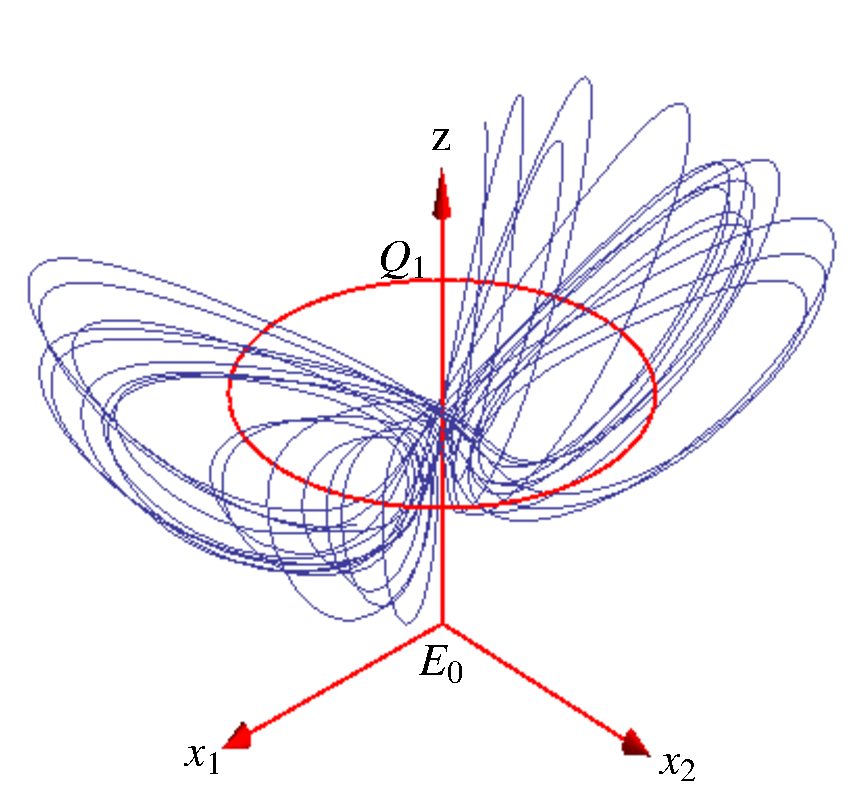
\includegraphics[width=0.40\textwidth, clip=true]{CLEchaotic}
  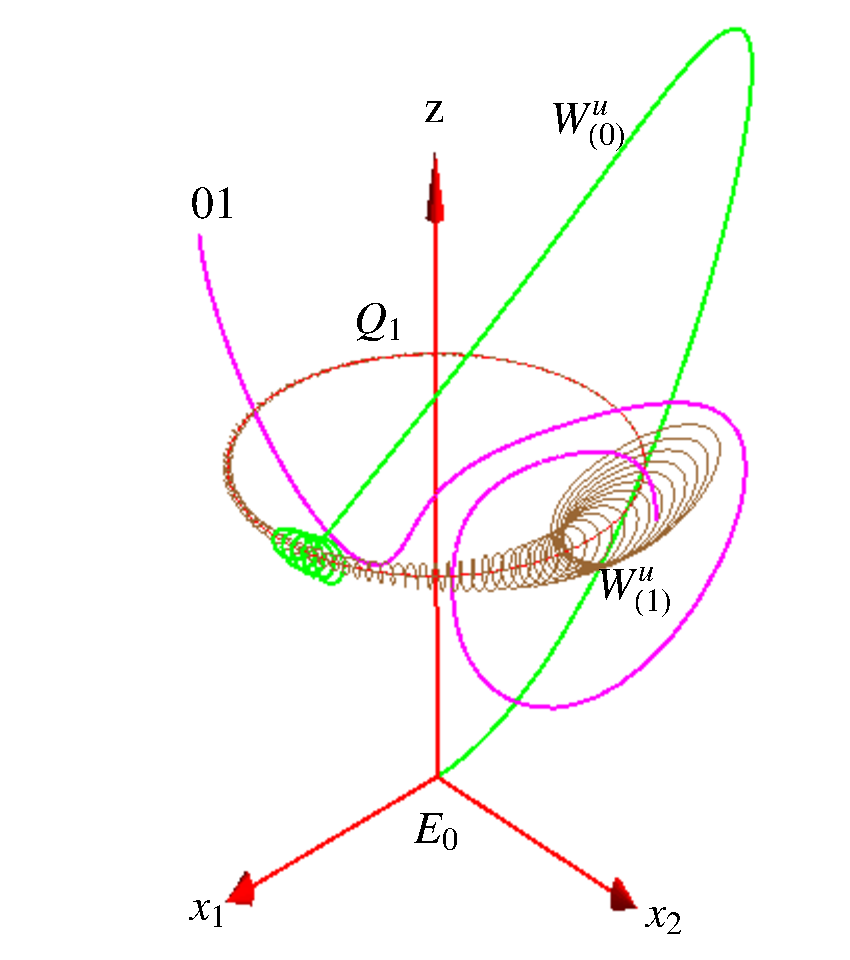
\includegraphics[width=0.40\textwidth, clip=true]{CLEcompact}
\end{center}
\caption{
\Statesp\ portrait of \cLf. Plotted are a generic chaotic trajectory (blue),
\eqv\
\EQV{0}, a representative of its unstable manifold (green),
\reqv\ \REQV{}{1} (red), its unstable manifold (brown), and
three repeats of the \cycle{01} \rpo.
}
\label{fig:CLE}
\end{figure}
%%%%%%%%%%%%%%%%%%%%%%%%%%%%%%%%%%%%%%%%%%%%%%%%%%%%%%%%%%%%
%
Why worry about continuous symmetries? \JFGedit{The visualization 
in \reffig{fig:CLE}} of typical long-time dynamics of \cLf\ suffices
to illustrate the effect a continuous symmetry has on
dynamics. A generic trajectory slowly `drifts' along the
direction of continuous symmetry while tracing a
Lorenz-butterfly like attractor. It is a mess.

\JFGedit{The} \CLe\ are a dynamical system with a continuous 
(but no discrete) symmetry, equivariant under the one-parameter
rotation group $\Un{1}\cong\SOn{2}$ acting by
\beq\label{eq:SO2cle}
	(x,\,y,\,z)\mapsto (
    e^{i\theta}x,\,e^{i\theta}y,\,z)\,,\ \theta\in[0,2\pi]
\,.
\eeq
Alternatively, substituting the Lie algebra generator
    \PC{is the sign standard? {\bf ES:} No. According
to Byron and Fuller, Mathematics of Classical and Quantum
Physics, which I find a very reliable and carefully written
book, what I use right now is the convention most physicists
use for \emph{active} tranformations. This I've also used
in thesis and I'd be happy to stick with this. With this choice
small angle, active rotations, are counterclockwise, so I've updated
our orientation condition as well.} 
\beq
 \Lg \,=\,   \left(\barr{ccccc}
    0  & -1 & 0  &  0 & 0  \\
    1  &  0 & 0  &  0 & 0 \\
    0  &  0 & 0  & -1 & 0  \\
    0  &  0 & 1  &  0 & 0 \\
    0  &  0 & 0  &  0 & 0
    \earr\right)
\ee{CLfLieGen}
acting on a 5-dim\-ens\-ion\-al space \refeq{eq:CLeR} into
\refeq{FiniteRot} yields the  $\Rls{5}$ representation of a
finite angle action \refeq{eq:SO2cle} of $\SOn{2}$
\beq
\LieEl(\gSpace) \,=\,  \left(\barr{ccccc}
  \cos \gSpace  & -\sin \gSpace  & 0 & 0 & 0 \\
  \sin \gSpace  &  \cos \gSpace  & 0 & 0 & 0 \\
 0 & 0 &  \cos \gSpace & -\sin \gSpace   & 0 \\
 0 & 0 &  \sin \gSpace &  \cos \gSpace   & 0 \\
 0 & 0 & 0             & 0               & 1
    \earr\right)
\,.
\ee{CLfRots}
We see that the linear action of \SOn{2}\
\JFGedit{on the \statesp\ of the \cLe\ } 
decomposes into the $m\!=\!0$ \Group-invariant
subspace ($z$-axis) and  the $m=1$ subspace of multiplicity 2.

The generator $\Lg$ is anti-hermitian,
$\Lg^\dagger = - \Lg$, and the group is compact, its
elements parametrized by $\gSpace \mbox{ mod } 2\pi$. Locally, at
$\ssp \in \pS$, the infinitesimal action of the group is
given by the group tangent field $\groupTan(\ssp) = \Lg \ssp
= (-x_2,x_1,-y_2,y_1,0)$. In other words, the flow induced by
the group action is normal to the radial direction in the
$(x_1,x_2)$ and $(y_1,y_2)$ planes, while the $z$-axis is left
invariant.

\JFGedit{The equivariance of the \cLf\ under $\SOn{2}$ rotations 
\refeq{CLfRots} can be verified} 
by substituting the Lie algebra generator
\refeq{CLfLieGen} and the \stabmat\ for \cLf\ \refeq{eq:CLeR},
  \beq
\Mvar =
  \left(\barr{ccccc}
    -\sigma    	& 0 		& \sigma & 0    &  0 \\
	0 	& -\sigma       & 0      & \sigma   &  0 \\
	\RerCLor-z  &     -\ImrCLor      & -1     & -e & -x_1 \\
	\ImrCLor     & \RerCLor-z       	& e  	& -1       & -x_2 \\
	y_1     & y_2           & x_1    & x_2      & -b
    \earr\right)
\,,
  \ee{CLeStabMat}
into the equivariance condition \refeq{inftmInv}.
For the parameter values \refeq{eq:CLeR} the flow
is strongly volume contracting,
\beq
\pde_i \pVeloc_i
 = \sum_{i=1}^{5} \Lyap_i(\ssp,t)
= -b -2(\sigma + 1)
= -24 - 2/3
    \,,
\ee{trA-ZM}

\JFGedit{The} \CLe\ \refeq{eq:CLe} were introduced by
Gibbon and McGuinness\rf{GibMcCLE82,FowlerCLE82} as a
low-dim\-ens\-ion\-al model of baroclinic instability in the
atmosphere. Ning and Haken\rf{NingHakenCLE90} have shown that
equations isomorphic to \JFGedit{the} \cLe\ also appear as a truncation of
Maxwell-Bloch equations describing a single mode, detuned,
ring laser. They set $e+\ImrCLor=0$ (see \refeq{eq:omegaCLE})
so that \SOn{2}-orbits of detuned \eqva\
exist\rf{FowlerCLE82}. Zeghlache and Mandel\rf{ZeMa85} also
use equations isomorphic to \cLe\ with $e+\ImrCLor=0$ in
their studies of detuned ring lasers. This choice is
`degenerate' in the sense that it leads to non-generic
bifurcations. As the existence of \reqva\ in systems with \SOn{2}
symmetry is the generic situation, we follow Bakasov and
Abraham\rf{BakasovAbraham93} who set $\ImrCLor=0$ and $e \neq
0$.

Here, however, we are not interested in the physical
applications of these equations; rather, we study them as a
simple example of a dynamical system with continuous (but no
discrete) symmetries, with a view of testing methods of
reducing the dynamics to a lower-dimensional \reducedsp.
    \PC{looks like one should also read \refref{Abraham95}; they
    report on various return maps}
We investigate
various ways of `quotienting' its \SOn{2} symmetry, and
reducing the dynamics to a 4-dim\-ens\-ion\-al \reducedsp. As
we shall show, the dynamics has a nice {\stretchf}
action, but that is totally masked by the continuous symmetry
drifts. We shall not rest until we attain the simplicity of
\reffig{fig:CLEmfReqb1}, and the bliss of 1-dim\-ens\-ion\-al
return map of \reffig{fig:CLEipRM}.
